% Options for packages loaded elsewhere
\PassOptionsToPackage{unicode}{hyperref}
\PassOptionsToPackage{hyphens}{url}
\PassOptionsToPackage{dvipsnames,svgnames*,x11names*}{xcolor}
%
\documentclass[
]{krantz}
\usepackage{lmodern}
\usepackage{amssymb,amsmath}
\usepackage{ifxetex,ifluatex}
\ifnum 0\ifxetex 1\fi\ifluatex 1\fi=0 % if pdftex
  \usepackage[T1]{fontenc}
  \usepackage[utf8]{inputenc}
  \usepackage{textcomp} % provide euro and other symbols
\else % if luatex or xetex
  \usepackage{unicode-math}
  \defaultfontfeatures{Scale=MatchLowercase}
  \defaultfontfeatures[\rmfamily]{Ligatures=TeX,Scale=1}
\fi
% Use upquote if available, for straight quotes in verbatim environments
\IfFileExists{upquote.sty}{\usepackage{upquote}}{}
\IfFileExists{microtype.sty}{% use microtype if available
  \usepackage[]{microtype}
  \UseMicrotypeSet[protrusion]{basicmath} % disable protrusion for tt fonts
}{}
\makeatletter
\@ifundefined{KOMAClassName}{% if non-KOMA class
  \IfFileExists{parskip.sty}{%
    \usepackage{parskip}
  }{% else
    \setlength{\parindent}{0pt}
    \setlength{\parskip}{6pt plus 2pt minus 1pt}}
}{% if KOMA class
  \KOMAoptions{parskip=half}}
\makeatother
\usepackage{xcolor}
\IfFileExists{xurl.sty}{\usepackage{xurl}}{} % add URL line breaks if available
\IfFileExists{bookmark.sty}{\usepackage{bookmark}}{\usepackage{hyperref}}
\hypersetup{
  pdftitle={Multimodal Deep Learning},
  colorlinks=true,
  linkcolor=Maroon,
  filecolor=Maroon,
  citecolor=Blue,
  urlcolor=Blue,
  pdfcreator={LaTeX via pandoc}}
\urlstyle{same} % disable monospaced font for URLs
\usepackage{longtable,booktabs}
% Correct order of tables after \paragraph or \subparagraph
\usepackage{etoolbox}
\makeatletter
\patchcmd\longtable{\par}{\if@noskipsec\mbox{}\fi\par}{}{}
\makeatother
% Allow footnotes in longtable head/foot
\IfFileExists{footnotehyper.sty}{\usepackage{footnotehyper}}{\usepackage{footnote}}
\makesavenoteenv{longtable}
\usepackage{graphicx,grffile}
\makeatletter
\def\maxwidth{\ifdim\Gin@nat@width>\linewidth\linewidth\else\Gin@nat@width\fi}
\def\maxheight{\ifdim\Gin@nat@height>\textheight\textheight\else\Gin@nat@height\fi}
\makeatother
% Scale images if necessary, so that they will not overflow the page
% margins by default, and it is still possible to overwrite the defaults
% using explicit options in \includegraphics[width, height, ...]{}
\setkeys{Gin}{width=\maxwidth,height=\maxheight,keepaspectratio}
% Set default figure placement to htbp
\makeatletter
\def\fps@figure{htbp}
\makeatother
\setlength{\emergencystretch}{3em} % prevent overfull lines
\providecommand{\tightlist}{%
  \setlength{\itemsep}{0pt}\setlength{\parskip}{0pt}}
\setcounter{secnumdepth}{5}
\usepackage{booktabs}
\usepackage{longtable}
\usepackage[bf,singlelinecheck=off]{caption}

\usepackage{framed,color}
\definecolor{shadecolor}{RGB}{248,248,248}

\renewcommand{\textfraction}{0.05}
\renewcommand{\topfraction}{0.8}
\renewcommand{\bottomfraction}{0.8}
\renewcommand{\floatpagefraction}{0.75}

\renewenvironment{quote}{\begin{VF}}{\end{VF}}
\let\oldhref\href
\renewcommand{\href}[2]{#2\footnote{\url{#1}}}

\makeatletter
\newenvironment{kframe}{%
\medskip{}
\setlength{\fboxsep}{.8em}
 \def\at@end@of@kframe{}%
 \ifinner\ifhmode%
  \def\at@end@of@kframe{\end{minipage}}%
  \begin{minipage}{\columnwidth}%
 \fi\fi%
 \def\FrameCommand##1{\hskip\@totalleftmargin \hskip-\fboxsep
 \colorbox{shadecolor}{##1}\hskip-\fboxsep
     % There is no \\@totalrightmargin, so:
     \hskip-\linewidth \hskip-\@totalleftmargin \hskip\columnwidth}%
 \MakeFramed {\advance\hsize-\width
   \@totalleftmargin\z@ \linewidth\hsize
   \@setminipage}}%
 {\par\unskip\endMakeFramed%
 \at@end@of@kframe}
\makeatother

\usepackage{makeidx}
\makeindex

\urlstyle{tt}

\usepackage{amsthm}
\makeatletter
\def\thm@space@setup{%
  \thm@preskip=8pt plus 2pt minus 4pt
  \thm@postskip=\thm@preskip
}
\makeatother

\frontmatter
\usepackage[]{natbib}
\bibliographystyle{apalike}

\title{Multimodal Deep Learning}
\author{}
\date{\vspace{-2.5em}2022-05-30}

\begin{document}
\maketitle

% you may need to leave a few empty pages before the dedication page

%\cleardoublepage\newpage\thispagestyle{empty}\null
%\cleardoublepage\newpage\thispagestyle{empty}\null
%\cleardoublepage\newpage
\thispagestyle{empty}

\begin{center}
\end{center}

\setlength{\abovedisplayskip}{-5pt}
\setlength{\abovedisplayshortskip}{-5pt}

{
\hypersetup{linkcolor=}
\setcounter{tocdepth}{0}
\tableofcontents
}
\hypertarget{preface}{%
\chapter*{Preface}\label{preface}}


\begin{figure}
\centering

\includegraphics{figures/by-nc-sa.png}
\caption{Creative Commons License}
\end{figure}

This book is licensed under the \href{http://creativecommons.org/licenses/by-nc-sa/4.0/}{Creative Commons Attribution-NonCommercial-ShareAlike 4.0 International License}.

\mainmatter

\hypertarget{foreword}{%
\chapter*{Foreword}\label{foreword}}


\emph{Author: Christoph Molnar}

This book is the result of an experiment in university teaching.
Each semester, students of the Statistics Master can choose from a selection of seminar topics.
Usually, every student in the seminar chooses a scientific paper, gives a talk about the paper and summarizes it in the form of a seminar paper.
The supervisors help the students, they listen to the talks, read the seminar papers, grade the work and then \ldots{} hide the seminar papers away in (digital) drawers.
This seemed wasteful to us, given the huge amount of effort the students usually invest in seminars.
An idea was born:
Why not create a book with a website as the outcome of the seminar?
Something that will last at least a few years after the end of the semester.
In the summer term 2019, some Statistics Master students signed up for our seminar entitled ``Limitations of Interpretable Machine Learning''.
When they came to the kick-off meeting, they had no idea that they would write a book by the end of the semester.

We were bound by the examination rules for conducting the seminar, but otherwise we could deviate from the traditional format.
We deviated in several ways:

\begin{enumerate}
\def\labelenumi{\arabic{enumi}.}
\tightlist
\item
  Each student project is part of a book, and not an isolated seminar paper.
\item
  We gave challenges to the students, instead of papers. The challenge was to investigate a specific limitation of interpretable machine learning methods.
\item
  We designed the work to live beyond the seminar.
\item
  We emphasized collaboration. Students wrote some chapters in teams and reviewed each others texts.
\end{enumerate}

\hypertarget{technical-setup}{%
\section*{Technical Setup}\label{technical-setup}}


The book chapters are written in the Markdown language.
The simulations, data examples and visualizations were created with R \citep{rlang}.
To combine R-code and Markdown, we used rmarkdown.
The book was compiled with the bookdown package.
We collaborated using git and github.
For details, head over to the \href{https://github.com/slds-lmu/seminar_multimodal_dl}{book's repository}.

\hypertarget{introduction}{%
\chapter{Introduction}\label{introduction}}

\emph{Author: }

\emph{Supervisor: }

\hypertarget{intro-about-the-seminar-topic}{%
\section{Intro About the Seminar Topic}\label{intro-about-the-seminar-topic}}

\hypertarget{outline-of-the-booklet}{%
\section{Outline of the Booklet}\label{outline-of-the-booklet}}

\hypertarget{chapter-1}{%
\chapter{Chapter 1}\label{chapter-1}}

\emph{Authors: Author 1, Author 2}

\emph{Supervisor: Supervisor}

\hypertarget{lorem-ipsum}{%
\section{Lorem Ipsum}\label{lorem-ipsum}}

Lorem ipsum dolor sit amet, consetetur sadipscing elitr, sed diam nonumy eirmod tempor invidunt ut labore et dolore magna aliquyam erat, sed diam voluptua. At vero eos et accusam et justo duo dolores et ea rebum. Stet clita kasd gubergren, no sea takimata sanctus est Lorem ipsum dolor sit amet. Lorem ipsum dolor sit amet, consetetur sadipscing elitr, sed diam nonumy eirmod tempor invidunt ut labore et dolore magna aliquyam erat, sed diam voluptua. At vero eos et accusam et justo duo dolores et ea rebum. Stet clita kasd gubergren, no sea takimata sanctus est Lorem ipsum dolor sit amet.

\citet{rlang}

\hypertarget{using-figures}{%
\section{Using Figures}\label{using-figures}}

\begin{figure}

{\centering 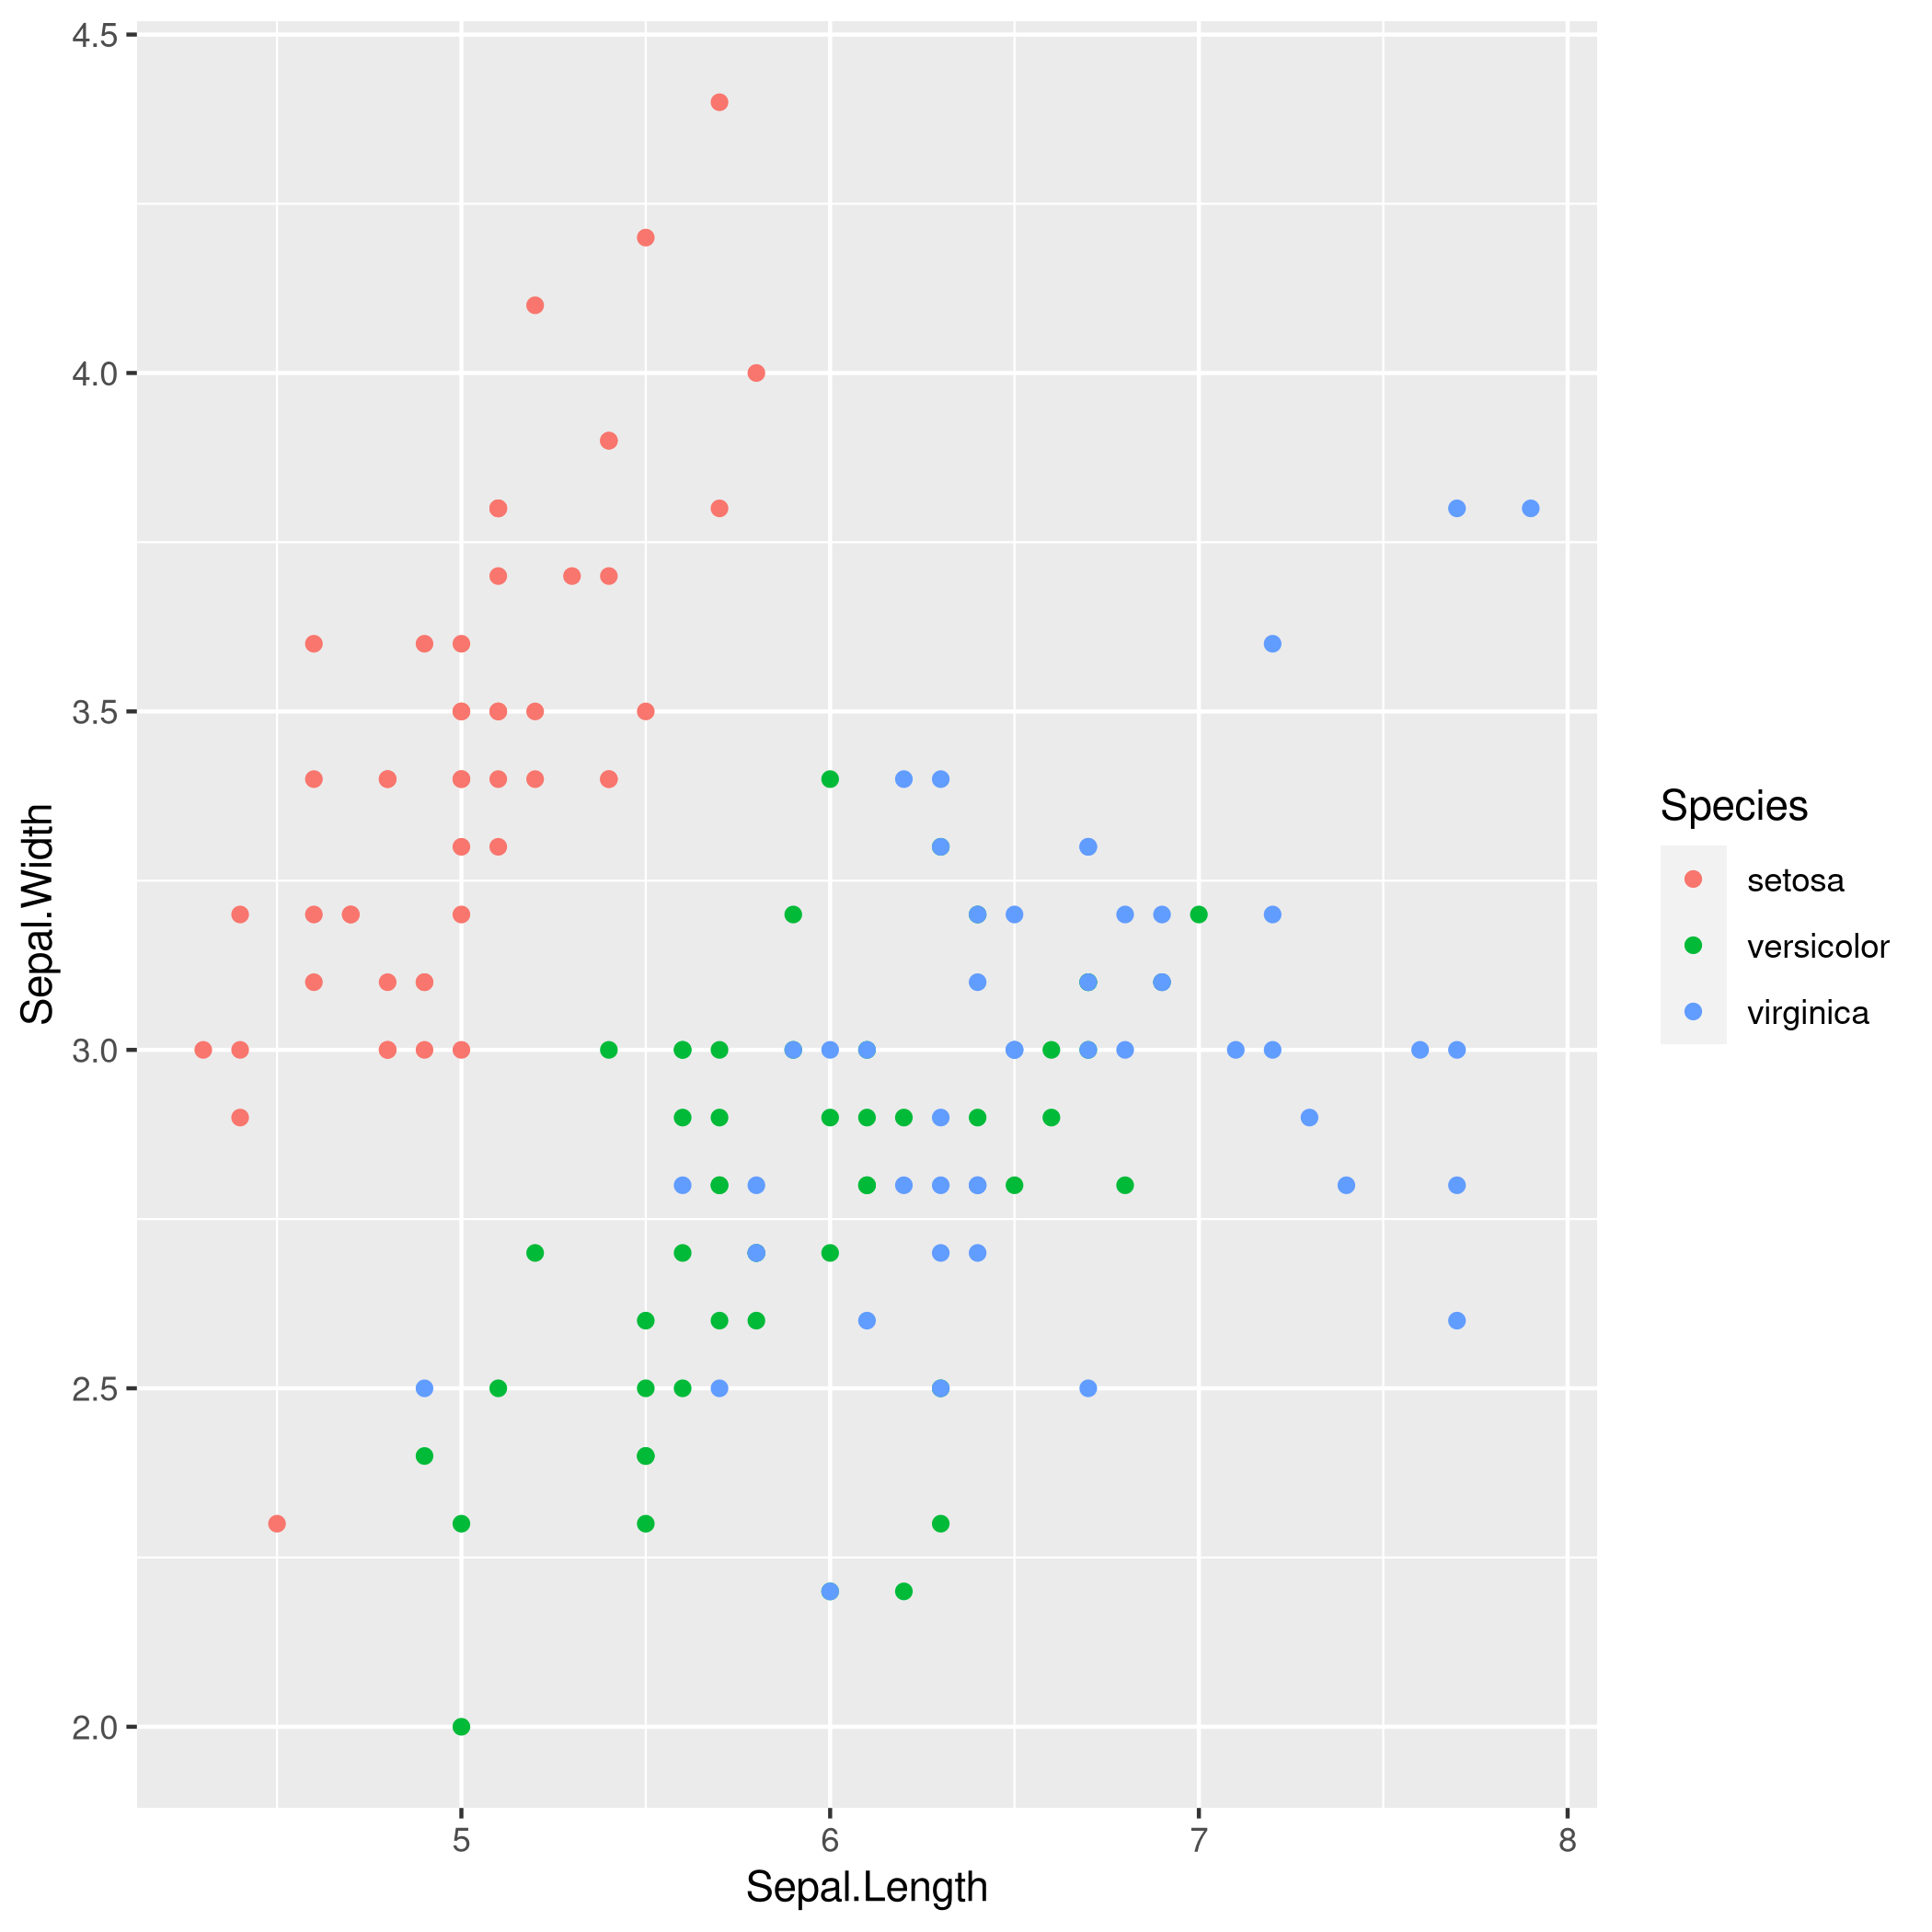
\includegraphics[width=0.8\linewidth]{figures/01-chapter1/ch01-figure01} 

}

\caption{This is the caption of the figure!}\label{fig:ch01-figure01}
\end{figure}



Referencing can be done by using the chunk label e.g.~\texttt{\textbackslash{}@ref(fig:ch01-figure01)} for \ref{fig:ch01-figure01}.

\textbf{NOTE!!!} Do not use underscores in chunk labels! This will crash the compilation \ldots{}

\hypertarget{using-tex}{%
\section{Using Tex}\label{using-tex}}

HTML rendering uses MathJax while pdf rendering uses LaTeX:

\[
f(x) = x^2
\]

\hypertarget{using-stored-results}{%
\section{Using Stored Results}\label{using-stored-results}}

\begin{tabular}{l|r|r|r|r}
\hline
  & Estimate & Std. Error & t value & Pr(>|t|)\\
\hline
(Intercept) & 2.1713 & 0.2798 & 7.760 & 0.0000\\
\hline
Sepal.Width & 0.4959 & 0.0861 & 5.761 & 0.0000\\
\hline
Petal.Length & 0.8292 & 0.0685 & 12.101 & 0.0000\\
\hline
Petal.Width & -0.3152 & 0.1512 & -2.084 & 0.0389\\
\hline
Speciesversicolor & -0.7236 & 0.2402 & -3.013 & 0.0031\\
\hline
Speciesvirginica & -1.0235 & 0.3337 & -3.067 & 0.0026\\
\hline
\end{tabular}

\hypertarget{title}{%
\chapter{title}\label{title}}

\emph{Author: }

\emph{Supervisor: }

\hypertarget{title-1}{%
\chapter{title}\label{title-1}}

\emph{Author: }

\emph{Supervisor: }

\hypertarget{title-2}{%
\chapter{title}\label{title-2}}

\emph{Author: }

\emph{Supervisor: }

\hypertarget{chapter-1-1}{%
\chapter{Chapter 1}\label{chapter-1-1}}

\emph{Authors: Author 1, Author 2}

\emph{Supervisor: Supervisor}

\hypertarget{lorem-ipsum-1}{%
\section{Lorem Ipsum}\label{lorem-ipsum-1}}

Lorem ipsum dolor sit amet, consetetur sadipscing elitr, sed diam nonumy eirmod tempor invidunt ut labore et dolore magna aliquyam erat, sed diam voluptua. At vero eos et accusam et justo duo dolores et ea rebum. Stet clita kasd gubergren, no sea takimata sanctus est Lorem ipsum dolor sit amet. Lorem ipsum dolor sit amet, consetetur sadipscing elitr, sed diam nonumy eirmod tempor invidunt ut labore et dolore magna aliquyam erat, sed diam voluptua. At vero eos et accusam et justo duo dolores et ea rebum. Stet clita kasd gubergren, no sea takimata sanctus est Lorem ipsum dolor sit amet.

\citet{rlang}

\hypertarget{using-figures-1}{%
\section{Using Figures}\label{using-figures-1}}

\begin{figure}

{\centering 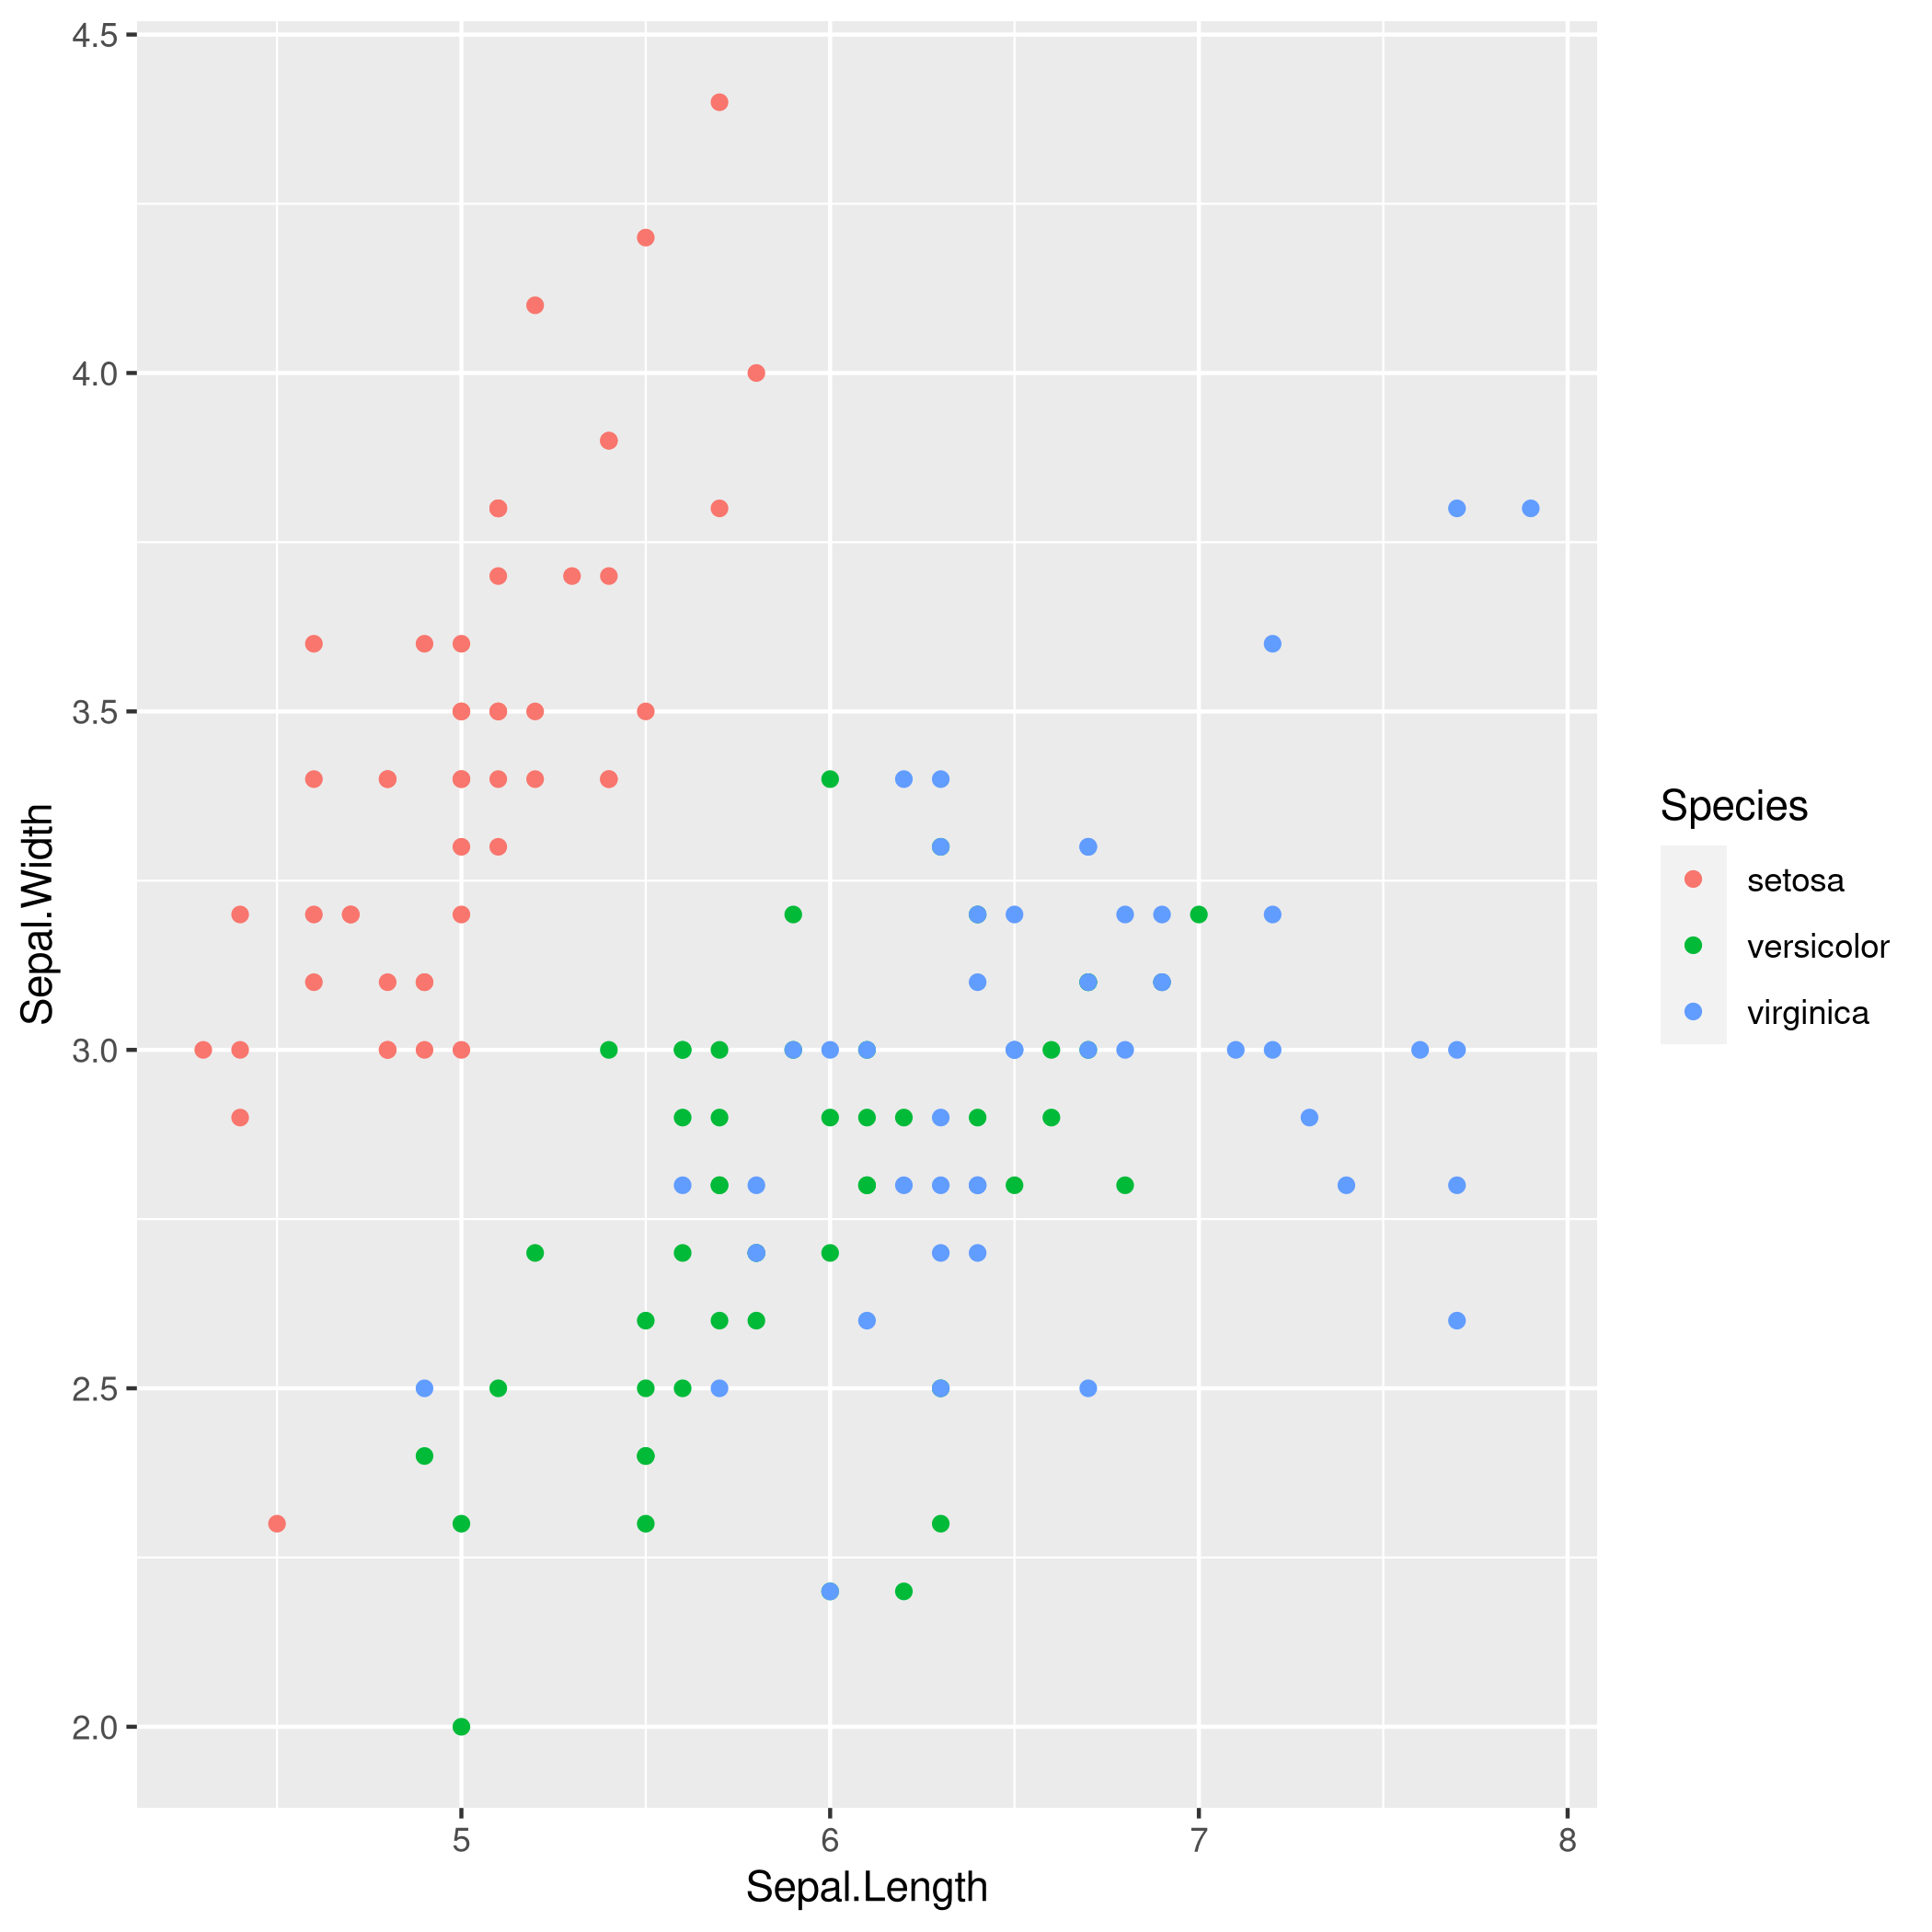
\includegraphics[width=0.8\linewidth]{figures/01-chapter1/ch01-figure01} 

}

\caption{This is the caption of the figure!}\label{fig:ch01-figure01-old}
\end{figure}

This is the caption of the figure! This is the caption of the figure!

Referencing can be done by using the chunk label e.g.~\texttt{\textbackslash{}@ref(fig:ch01-figure01)} for \ref{fig:ch01-figure01}.

\textbf{NOTE!!!} Do not use underscores in chunk labels! This will crash the compilation \ldots{}

\hypertarget{using-tex-1}{%
\section{Using Tex}\label{using-tex-1}}

HTML rendering uses MathJax while pdf rendering uses LaTeX:

\[
f(x) = x^2
\]

\hypertarget{using-stored-results-1}{%
\section{Using Stored Results}\label{using-stored-results-1}}

\begin{tabular}{l|r|r|r|r}
\hline
  & Estimate & Std. Error & t value & Pr(>|t|)\\
\hline
(Intercept) & 2.1713 & 0.2798 & 7.760 & 0.0000\\
\hline
Sepal.Width & 0.4959 & 0.0861 & 5.761 & 0.0000\\
\hline
Petal.Length & 0.8292 & 0.0685 & 12.101 & 0.0000\\
\hline
Petal.Width & -0.3152 & 0.1512 & -2.084 & 0.0389\\
\hline
Speciesversicolor & -0.7236 & 0.2402 & -3.013 & 0.0031\\
\hline
Speciesvirginica & -1.0235 & 0.3337 & -3.067 & 0.0026\\
\hline
\end{tabular}

\hypertarget{title-3}{%
\chapter{title}\label{title-3}}

\emph{Author: }

\emph{Supervisor: }

\hypertarget{title-4}{%
\chapter{title}\label{title-4}}

\emph{Author: }

\emph{Supervisor: }

\hypertarget{title-5}{%
\chapter{title}\label{title-5}}

\emph{Author: }

\emph{Supervisor: }

\hypertarget{title-6}{%
\chapter{title}\label{title-6}}

\emph{Author: }

\emph{Supervisor: }

\hypertarget{title-7}{%
\chapter{title}\label{title-7}}

\emph{Author: }

\emph{Supervisor: }

\hypertarget{title-8}{%
\chapter{title}\label{title-8}}

\emph{Author: }

\emph{Supervisor: }

\hypertarget{chapter-2-multimodal-architectures}{%
\chapter{Chapter 2 Multimodal architectures}\label{chapter-2-multimodal-architectures}}

\emph{Authors: Luyang Chu, Karol Urbanczyk, Giacomo Loss, Max Schneider, Steffen Jauch-Walser}
\emph{Supervisor: Christian Heumann}

\hypertarget{introduction-1}{%
\section{Introduction}\label{introduction-1}}

Multimodal learning refers to the process of learning representations from different types of input modalities, such as image data, text or speech.
Due to methodological breakthroughs in the fields of Natural Language Processing (NLP) as well as Computer Vision (CV), in recent years multimodal models have gained increasing attention as they are able to strengthen predictions and better emulate the way humans learn.
This chapter focuses on discussing images and text as input data.
The remainder of the chapter is structured as follows:

The first part ``Image2Text'' discusses how transformer-based architectures improve meaningful captioning for complex images using a new large scale, richly annotated dataset COCO \citep{mccoco, cornia2020m2}.
Whether it is seeing a photograph and describing it or parsing a complex scene and describing its context, it is not a difficult task for humans.
But it is much more complex and challenging for computers.
We start with focusing on images as input modalities.
In 2014 Microsoft COCO was developed with a primary goal of advancing the state-of-the-art (SOTA) in object recognition by diving deeper into a broader question of scene understanding \citep{mccoco}.
COCO stands for Common Objects in Context.
It addresses three core problems in scene understanding: object detection (non-iconic views), segmentation, and captioning.
For tasks like machine translation and language understanding in NLP, transformer-based architecture is widely used.
However, the potential of these applications in the multi-modal context has not been fully covered.
With the help of the COCO dataset, a transformer-based architecture: Meshed-Memory Transformer for Image Captioning (\(M^2\)) will be introduced to improve both image encoding and the language generation steps \citep{cornia2020m2}.
The performance of the (\(M^2\)) Transformer and different fully-attentive models will be evaluated and compared on the COCO dataset.

Next, in ``Text2Image'', the idea of incorporating textual input in order to generate visual representations is described.
Current advancements in this field have been made possible largely due to recent breakthroughs in NLP, which first allowed for learning contextual representations of text.
Transformer-like architectures are being used to encode the input into embedding vectors, which are later helpful in guiding the process of image generation.
The chapter looks into details and discusses two SOTA model architectures by OpenAI, which both condition on text representations.
Surprisingly, none of them uses a GAN approach - a method which probably has been seen as the go-to idea for image generation over the last years.
The first model is DALL-E \citep{ramesh2021dalle}, which essentially combines Variational Encoder (VAE) with Autoregressive Transformer.
In the first step, VAE is being trained to learn downsized image representations.
Such embeddings are concatenated with text embeddings into one text-image pair input.
However, both of them use different dimensionality and vocabulary size.
In the second step, the transformer is trained on a next token prediction task given these data pairs.
Finally, at inference time, the model is able to generate images in the following way:

\begin{enumerate}
\def\labelenumi{\arabic{enumi}.}
\tightlist
\item
  Encode text input into text embedding
\item
  Use trained transformer from step 2 to generate image embedding
\item
  Use VAE from step 1 to generate image from image embedding
\end{enumerate}

The next approach to text-to-image generation is a GLIDE model \citep{nichol2021glide}.
GLIDE stands for Guided Language to Image Diffusion for Generation and Editing.
Its idea is to use Diffusion Models.
In its core, Diffusion Model is a simple idea -- random noise is being added to the image in an iterative fashion, and then model learns how to reconstruct this image.
In the case of GLIDE this learning process is conditioned on the text prompt, which is first passed through a transformer.
Both models differ in their results.
While DALL-E's resulting images might have been overwhelming back in the beginning of 2021, GLIDE is thought to significantly improve on photorealism and resolution the generated images.
Since the field has already seen further improvements following GLIDE, these new developments are also going to be mentioned in the chapter.

The third part, ``Images supporting Language Models'', deals with the integration of visual elements in pure textual language models.
Distributional semantic models such as Word2Vec and BERT assume that the meaning of a given word or sentence can be understood by looking at how (in which context) and when the word or the sentence appear in the text corpus, namely from its ``distribution'' within the text.
But this assumption has been historically questioned, because words and sentences must be grounded in other perceptual dimensions in order to understand their meaning \citep[see for example the ``symbol grounding problem'';][]{harnad1990symbol}.
For these reasons, a broad range of models has been developed with the aim to improve pure language models, leveraging on the addition of other perceptual information, such as visual ones.
This subchapter focuses in particular on the integration of visual elements (images) to support pure language models for various tasks at the word-level and sentence-level.
The starting point is always a language model, on which visual representations (extracted often with the help of large pools of images like MS COCO, see chapter ``Img2Text'' for further references) are to be ``integrated''.
But how?
There has been proposed a wide range of solutions:
On one side of the spectrum, textual elements and visual ones are learned separately and then ``combined'' together whereas on the other side, the learning of textual and visual features takes place simultaneously/jointly.

\begin{figure}

{\centering 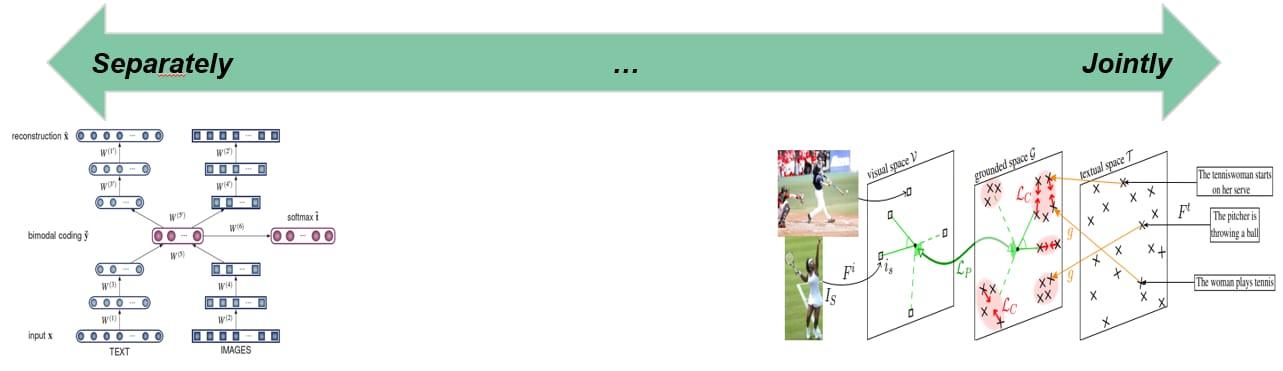
\includegraphics[width=1\linewidth]{figures/02-chapter2/Img_Ch_Intro} 

}

\caption{Left, Silberer et al., 2014: stacked autoencoders to learn higher-level embeddings from textual and visual modalities, encoded as vectors of attributes. Right, Bordes et al., 2020: textual and visual information fused in an Intermediate space denoted as “grounded space”; the “grounding objective function” is not applied directly on sentence embeddings but trained on this intermediate space, on which sentence embeddings are projected.}\label{fig:unnamed-chunk-1}
\end{figure}

For example, \citet{silberer2012grounded} implement a model where a one-to-one correspondence between textual and visual space is assumed.
Text and visual representations are passed to two separate unimodal encoders and both outputs are then fed to a bimodal autoencoder.
On the other side, \citet{bordes2020incorporating} propose a ``text objective function'' whose parameters are shared with an additional ``grounded objective function''.
The training of the latter takes place in what the authors called a ``grounded space'', which allows to avoid the one-to-one correspondence between textual and visual space.
These are just introductory examples and between these two approaches there are many shades of gray (maybe more than fifty\ldots).
These models exhibit in many instances better performance than pure language models, but they still struggle on some aspects, for example when they deal with abstract words and sentences.

Afterwards, in ``Text supporting Image Models'', approaches where natural language is used as supervision for CV models are described.
Intuitively these models should be more powerful compared to models supervised solely by manually labeled data, simply because there is much more training data available.
An important example for this is the CLIP model \citep{radford2021learning} with its new dataset WIT (WebImageText) comprising 400 million text-image pairs scraped from the internet.\\
Similar to ``Text2Image'' the recent successes in NLP have inspired new approaches in this field.
Most importantly pre-train methods, which directly learn from raw text \citep[e. g. GPT-n, Generative Pre-trained Transformer;][]{brown2020language}.
So, CLIP stands for Contrastive Language-Image Pre-training.
A transformer-like architecture is used for jointly pre-training a text encoder and an image encoder.
For this the contrastive goal to correctly predict which natural language text pertains to which image inside a certain batch, is employed.
Training this way turned out to be more efficient than to generate captions for images.\\
This leads to a flexible model, which at test time uses the learned text encoder as a ``zero-shot'' classifier on embeddings of the target dataset's classes.
The model, for example, can perform optical character recognition, geo-location and action-recognition.
Performance-wise CLIP can be competitive with task-specific supervised models, while never seeing an instance of the specific dataset before.
This suggests an important step towards closing the ``robustness gap'', where machine learning models fail to meet the expectations set by their previous performance -- especially on ImageNet test-sets -- on new datasets.

Finally, ``Text plus Images'' discusses how text and image inputs can be incorporated into a single unifying framework in order to get closer to a general self-supervised learning model.
There are two key advantages that make such a model particularly interesting.
Similar to models mentioned in previous parts, devoid of human labelling, self-supervised models don't suffer from the same capacity constraints as regular supervised learning models.
Nevertheless, while there have been notable advances in dealing with different modalities, it is often unclear to which extend a model structure generalizes across different modalities.
Rather than potentially learning modality-specific biases, a general multipurpose framework can help increase robustness while also simplifying the learner portfolio and thereby better emulating human learning processes.\\
Data2vec \citep{baevski2022data2vec} is a new multimodal self-supervised learning model which uses a single framework for either speech, NLP or computer vision.
This is in contrast to earlier models which used different algorithms for different modalities.
The core idea of data2vec, developed by MetaAI, is to predict latent representations of the full input data based on a masked view of the input in a self-distillation setup using a standard transformer architecture \citep{baevski2022data2vec}.
As a result, the main improvement is in the framework, not the underlying models themselves.
For example, the transformer architecture follows \citet{vaswani2017attention}.
Transformers have several advantages over CNNs, such as encoding the relative position of features (citation needed).
The central building block of the data2vec framework is a student-teacher structure that allows the learning process to occur without supervision.
To achieve this, inputs serve both as training data and as learning targets by being masked.
A key issue to be aware of is model collapse, i.e the model collapsing into a constant representation.
Normalization helps prevent that, as well as the domination of certain layers with high norm.
The encoding, normalization and masking strategies are modality-specific.
However, the learning objective remains the same across all modalities.
The model is trained to predict the model representation of the original unmasked training sample.
As a result of the use of self-attention in creating teacher representations, the data2vec model works with continuous and contextualized targets which are richer in information than a fixed set of targets based on local context as used in most prior work.
On top of that, working with latent representations of the network itself can be seen as a simplification of many prior modality-specific models \citep{baevski2022data2vec}.
As far as the results are concerned, data2vec is effective in all three modalities.
It sets new SOTA scores on computer vision, speech recognition as well as speech learning benchmarking sets.

\hypertarget{title-9}{%
\chapter{title}\label{title-9}}

\emph{Author: }

\emph{Supervisor: }

\hypertarget{title-10}{%
\chapter{title}\label{title-10}}

\emph{Author: }

\emph{Supervisor: }

\hypertarget{title-11}{%
\chapter{title}\label{title-11}}

\emph{Author: }

\emph{Supervisor: }

\hypertarget{title-12}{%
\chapter{title}\label{title-12}}

\emph{Author: }

\emph{Supervisor: }

\hypertarget{title-13}{%
\chapter{title}\label{title-13}}

\emph{Author: }

\emph{Supervisor: }

\hypertarget{epilogue}{%
\chapter{Epilogue}\label{epilogue}}

\emph{Author: }

\hypertarget{test}{%
\section{test}\label{test}}

\hypertarget{acknowledgements}{%
\chapter{Acknowledgements}\label{acknowledgements}}

The most important contributions are from the students themselves.
The success of such projects highly depends on the students.
And this book is a success, so thanks a lot to all the authors!
The other important role is the supervisor.
Thanks to all the supervisors who participated!
Special thanks to \href{https://www.misoda.statistik.uni-muenchen.de/personen/professoren/heumann/index.html}{Christian Heumann} and \href{https://www.statistik.uni-muenchen.de/personen/professoren/bischl/index.html}{Bernd Bischl} who enabled us to conduct the seminar in such an experimental way, supported us and gave valuable feedback for the seminar structure.
Thanks a lot as well to the entire \href{https://www.statistik.uni-muenchen.de/}{Department of Statistics} and the \href{http://www.en.uni-muenchen.de/index.html}{LMU Munich} for the infrastructure.

The authors of this work take full responsibilities for its content.

  \bibliography{book.bib,packages.bib}

\backmatter
\printindex

\end{document}
